\chapter{Machine Learning}

\section{\textit{Lun 3 novembre - Lezione 12}}
\section{Introduction to Machine Learning}

\subsection{Topics}

\begin{enumerate}
	\item Introduction to machine learning
		\begin{enumerate}
			\item Basic concepts: loss, overfit, underfit
			\item Examples of linear regression, boosted decision trees
			\item Exercise with colab, numpy, scikit
		\end{enumerate}
	\item Deep Neural Networks
			\begin{enumerate}
			\item Basic FeedForward networks and backpropagation
			\item Importance of depth, gradient descent, optimizers
			\item Introduction to tools and first exercises
			\end{enumerate}
	\item Convolutional and Recurrent networks
		\begin{enumerate}
			\item Reduction of complexity with invariance: RNN and CNN
			\item CNN exercise
		\end{enumerate}
	\item Autoencoders and Generative Adversarial Networks
		\begin{enumerate}
			\item GAN exercises
		\end{enumerate}
	\item Graph Neural Networks
		\begin{enumerate}
			\item PointCloud exercise
		\end{enumerate}
\end{enumerate}

\subsection{Machine Learning Basics}
\textbf{Wikipedia:} Machine learning (ML) is a field of inquiry devoted to understanding and building methods that \textit{'learn'}, that is, methods that leverage data to improve performance on some set of tasks. It is seen as a part of \textit{artificial intelligence}. Machine learning algorithms build a model based on sample data, known as training data, in order to make predictions or decisions \textbf{without being explicitly programmed to do so}. Machine learning algorithms are used in a wide variety of applications, such as in medicine, email filtering, speech recognition, and computer vision, where it is difficult or unfeasible to develop conventional algorithms to perform the needed tasks.\\

Noi siamo abituati a dare al computer degli ordini imperativi.\\

In experimental and applied physics examples are everywhere...
\begin{itemize}
	\item Particle identification and kinematic measurement
	\item Signal to background discrimination (BDT and DNN are very popular in HEP experiments)
	\item Computer assisted processing of medical exams (ECG, CT, etc...)
	\item Processing of astrophysics data
\end{itemize}

\subsection{Types of typical ML problems}


\begin{itemize}
	\item \textbf{Classification:} which category a given input belongs to. 
	\item \textbf{Regression:} value of a real variable given the input.
	\item \textbf{Clustering:} group similar samples
	\item \textbf{Anomaly detection:} identify inputs that are “different” from the others
	\item \textbf{Generation/synthesis of samples:} produce new samples, similar to the original data, starting from noise/random numbers
	\item \textbf{Denoising:} remove noise from an input dataset
	\item \textbf{Transcriptions:} describe in some language the input data
	\item \textbf{Translations:} translate between languages
	\item \textbf{Encoding and decoding:} transform input data to a different representation
	\item ...many more...
\end{itemize}

\subsection{Function approximation}

The goal of a ML algorithm is to approximate an unknown function (often related to some Probability Density Function of the data) given some example data.\\
The function is often $ f(\textbf{x}): R^n \rightarrow R^m$ (in many simple problems $m=1$)
\begin{itemize}
	\item In\textbf{classification} we try to approximate the probability for each example, given the inputs represented as a vector \textbf{x}, to belong to a given category (y) (e.g. the probability to be a LHC Higgs signal event vs a Standard Model background one)
	\item In \textbf{regression} we approximate the function that given the inputs (x) returns the value of the variable to predict (y) (e.g. given the data read from some particle detectors, estimate the particle energy).
\end{itemize}

\begin{figure}[ht]
	\centering
	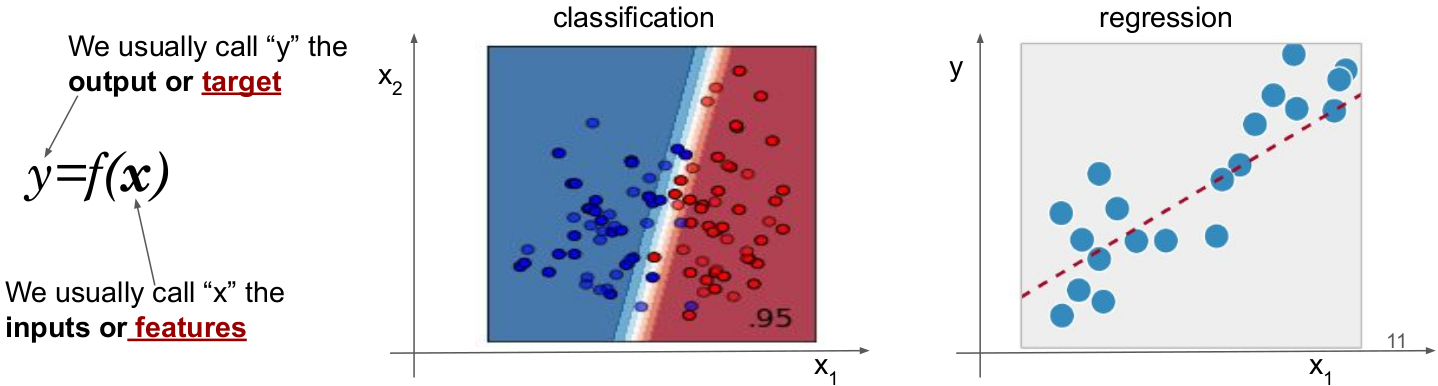
\includegraphics[width=1\textwidth]{figure_ml/function_approx.png}
\end{figure}
\FloatBarrier

\subsection{Model and Hyper-parameters}
A model for the functions that can be used to approximate the “f(x)” must be defined. The model can be something simple (e.g. sum of polynomials up to degree N) or more complex (e.g. all the functions that could be coded in M lines of C++).\\
Different ML techniques are based on different “models”:
\begin{itemize}
	\item Each technique (“class of model”) further allow to specify the exact model
	\item The parameters describing the exact model are called “hyper-parameters” (e.g. the degree N of the polynomial, or the maximum number of C++ line M can be considered hyper
	parameters)
\end{itemize}

We will see example of techniques with different models and complexity: (Linear regression, Decision trees, Principal Component Analysis, Nearest Neighbor, Artificial Neural Networks).

\subsection{Parameters}

A specific model typically have parameters (e.g. the coefficients of the polynomials or the characters of the 10 lines of C++).
Parameters are what we learn from data in the “training phase”.
Different models or similar model with different hyper-parameters settings have different n.d.o.f. in the parameters phase space.
\begin{equation*}
	y(x) = ax + bx^2 + cx^3 + d \qquad \qquad	\text{(a, b, c, d are the parameters)}
\end{equation*}

I parametri sono la cosa che voglio imparare nella fase di training. Mentre gli iperparametri li fisso prima di allenare il modello facendogli vedere i dati, i parametri sono invece proprio quelli che imparo.

\section{Objective function}
DObbiamo stabilire una metrica per dire quanto è buona la nostra approssimazione, dati gli esempi su ci ci stamo allenando.\\

A goal for what is “a good approximation” have to be defined This is called objective function (or loss function or error function …) Is a function that returns higher(or lower) value depending how good or bad the approximation is. Loss functions have to be minimized.\\
Examples of loss functions:
\begin{itemize}
	\item Classification problems: binary cross entropy
	\item Regression problems: Mean Square Error (i.e. the chi2 with sigma=1, I hope you are not surprised by this choice!)
\end{itemize}

The process is not very different from a typical phys-lab1 chi2 fit… but the number
of parameters can be several orders of magnitude larger ($10^3$ to $10^6$).

\subsubsection{Objective function: binary cross entropy}
In classification problems the function to approximate is typically $R^n \rightarrow [0,1]$, Where, for example, 0 means background and 1 means signal.\\
The binary cross entropy is defined as follows ($\hat{y}_i$ is the output of the classifier)
 
\begin{figure}[h]
	\centering
	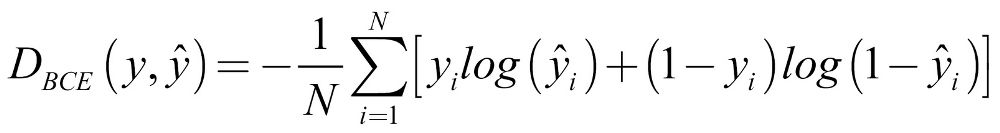
\includegraphics[width=0.5\textwidth]{figure_ml/D_bce.png}
\end{figure}
\FloatBarrier
The above function has large value when an example with y=1 is classified as 
a  $\hat{y}_i \sim 0$ and no loss when $\hat{y}_i \sim 1$. Viceversa if y=0 …\\
Minimizing the binary cross-entropy we maximize the likelihood in a process with 0/1 outcome (where the output of the function is interpreted as a probability).
 
\begin{figure}[h]
	\centering
	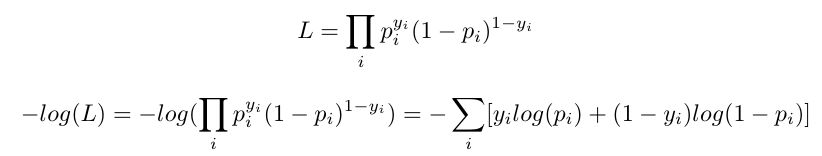
\includegraphics[width=0.65\textwidth]{figure_ml/L_bce.png}
\end{figure}
\FloatBarrier

\subsection{Learning / Training}
For a given model, and given set of hyper-parameters, how do we infer the parameters that minimize the objective function? The idea of ML is to get the parameters from “data” in a so called “training” step. Each ML technique has a different approach to training.\\
Different types of training:
\begin{itemize}
	\item \textbf{Supervised}: i.e. for each example we know the correct answer
	\item \textbf{Unsupervised}: we do not know “what is what”, we ask the ML algorithm to learn the probability density function of the examples in the features (i.e. the inputs!) space
	\item \textbf{Reinforcement learning}: have agents playing a punishment/reward game
\end{itemize}

\subsubsection{Supervised learning}

We want to teach something we (the supervisors) already know (at least on the training samples). For each example we need to have the “right answer” / “truth”, for example:

\begin{itemize}
	\item Labels telling if a given example signal or background, typically $y \in{0,1}$ (e.g. 0=background, 1=signal)
	\item Labels classifying the content of an image (multiple labels are possible)
	\item One-hot encoding used when multiple categories are possible:
		\begin{itemize}
			\item y=[0 1 0 0] means an element of the “2nd class”, y=[0 0 0 1] means an element of the “4th class”
			\item Much better than $y\in {0,1,2,3}$ if class “2” has no reason to be closer to “3” than to “0”
			\item Allows interpretation of the output (e.g. [0.1 0.3 0.06 0.001 ] as the probability to belong to each of the classes
			\item Allow for multi labeling (i.e. one sample can be belong to more than one category)
		\end{itemize}
	\item In regression problems the “truth” is the “correct values” of some quantity
		\begin{itemize}
			\item e.g. generated energy of a particle in a detector simulation
		\end{itemize}
\end{itemize}

Sample can be labelled in various ways:
\begin{itemize}
	\item Humans labelling existing data
	\item Data being “generated” from known functions (e.g. simulations)
\end{itemize}

Learn the probability of the label y, given the input \textbf{x}, i.e. P(y|\textbf{x})

\begin{figure}[ht]
	\centering
	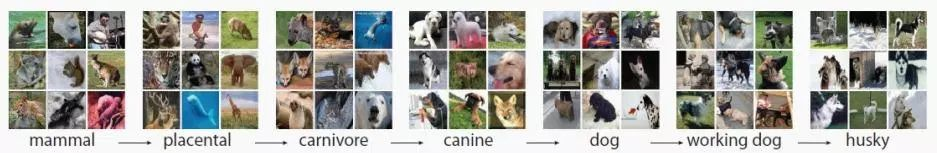
\includegraphics[width=1\textwidth]{figure_ml/supervised_learning.png}
\end{figure}
\FloatBarrier

\begin{figure}[ht]
	\centering
	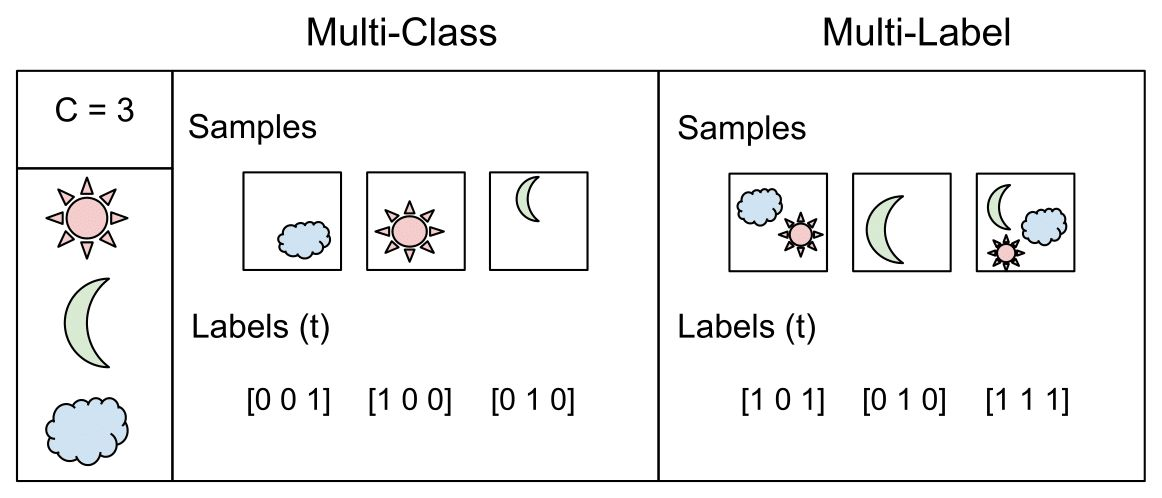
\includegraphics[width=0.4\textwidth]{figure_ml/multi_class.png}
\end{figure}
\FloatBarrier

\subsubsection{Unsupervised learning}

\begin{wrapfigure}{r}{0.5\textwidth}
	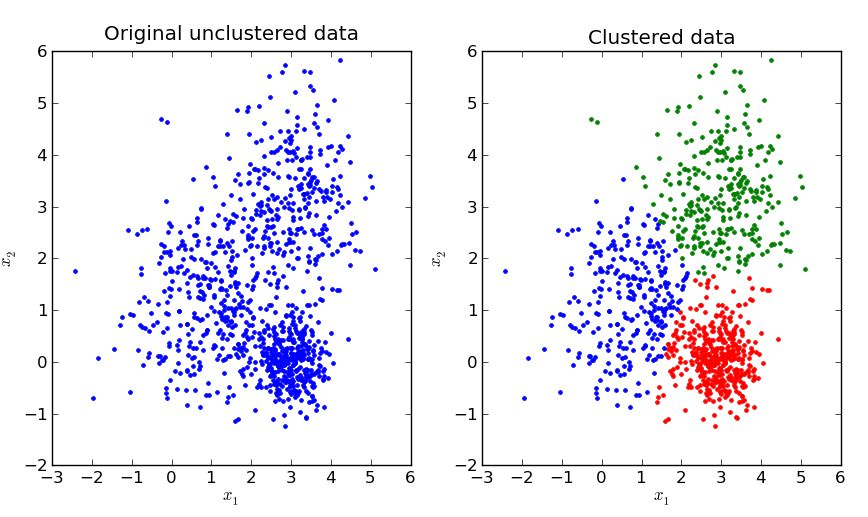
\includegraphics[width=0.5\textwidth]{figure_ml/unsupervised.png}
\end{wrapfigure} 

Often we do not have labels (or we have labels only for few data points). Unsupervised learning techniques allow to train networks that can perform
similar tasks as the supervised ones, e.g.

\begin{itemize}
	\item Classification of “common” patterns (clustering)
	\item Dimensionality reduction, compression
	\item Prediction of missing inputs
	\item Anomaly detection
\end{itemize}



In practice learn the Probability Density Function of the data, independently of any “label” variable, i.e. P(\textbf{x})

\subsubsection{Supervised vs unsupervised}

Supervised and unsupervised are not as different as one would imagine, in fact.\\
Unsupervised P(\textbf{x}) can be seen as n supervised problems, one for each feature of the input vector

\begin{figure}[ht]
	\centering
	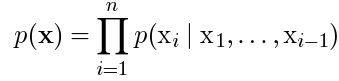
\includegraphics[width=0.4\textwidth]{figure_ml/s_vs_u.png}
\end{figure}
\FloatBarrier

Supervised P(y | \textbf{x}) can also be computed, if we treat y as an “\textbf{x}” in unsupervised learning deriving hence $p(\textbf{x},y)$
, as


\begin{figure}[ht]
	\centering
	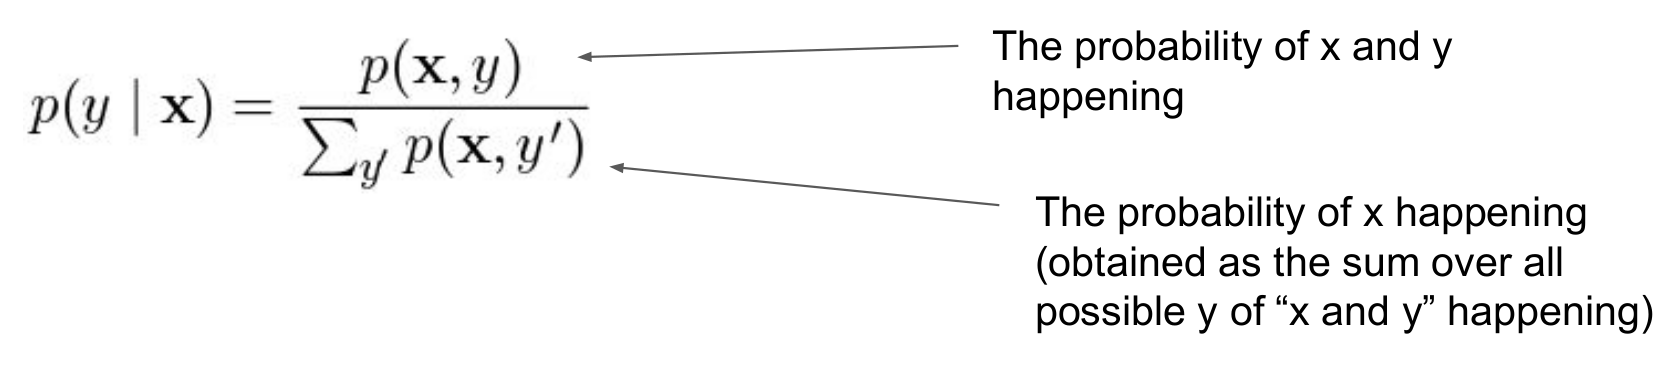
\includegraphics[width=0.8\textwidth]{figure_ml/s_vs_u2.png}
\end{figure}
\FloatBarrier

\subsubsection{Reinforcement learning (not covered in this lectures)}
\begin{wrapfigure}{r}{0.5\textwidth}
	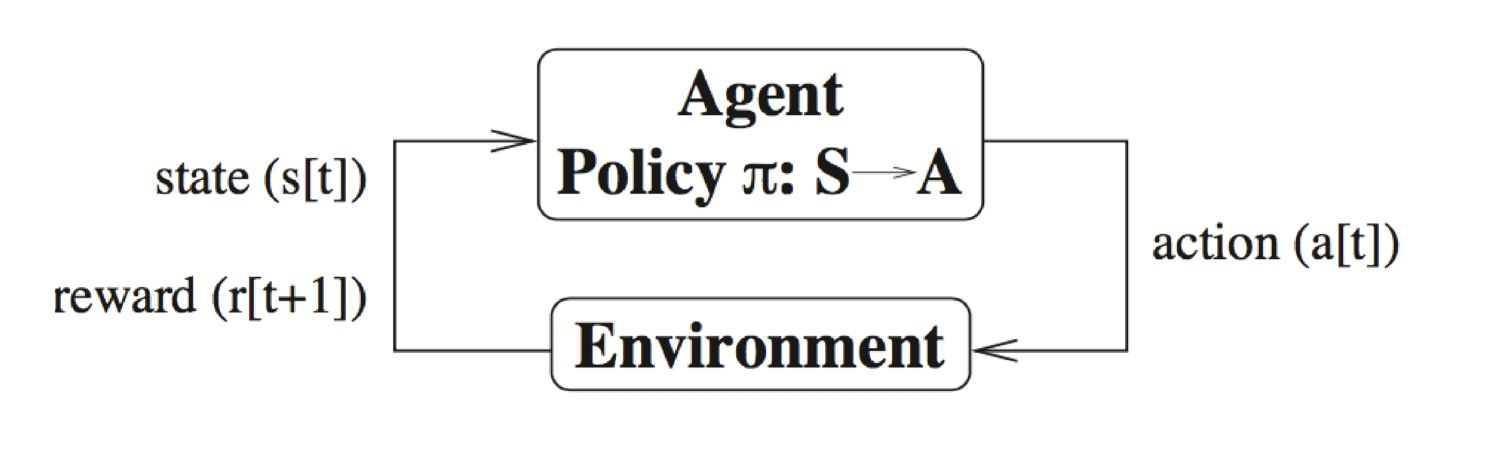
\includegraphics[width=0.5\textwidth]{figure_ml/reinforcement_learning.png}
\end{wrapfigure} 

Applies to “agents” acting in an “environment” that updates their state.\\
It is similar to supervised learning as a “reward” has to be calculated. The supervisor anyhow doesn’t necessarily know what is the best action to perform in a given state to interact with the environment, it just computes the final reward.\\
Learn to make best decision in a given situation
\begin{itemize}
	\item The right move in chess or go match
	\item Drive a car in the traffic
	\item Etc.
\end{itemize}


\subsection{Capacity and representational power}

\begin{wrapfigure}{r}{0.3\textwidth}
	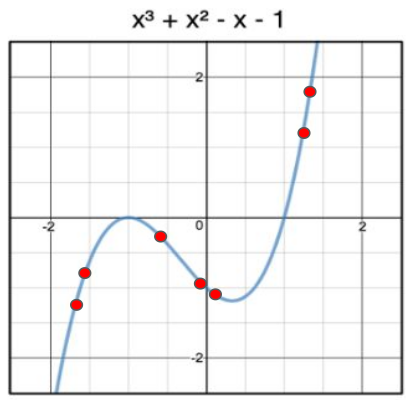
\includegraphics[width=0.3\textwidth]{figure_ml/capacity.png}
\end{wrapfigure} 

Different models (i.e. ML techniques/hyper-parametersvalues) allow to represent different type of functions.
Models with more free parameters typically can approximate a larger number
of functions (or can better approximate a given function) => higher capacity.
Remember: we do not know the actual function to approximate, we just want
to learn from examples.
With limited samples we have a tradeoff to
handle: accuracy in representation vs generalization of the results.\\


\noindent
\textbf{Underfitting:} the sample is badly represented.\\
\textbf{Overfitting} / Appropriate capacity are less obvious to define. (Lack of “generalization” $\rightarrow$ overfitting).

\begin{figure}[ht]
	\centering
	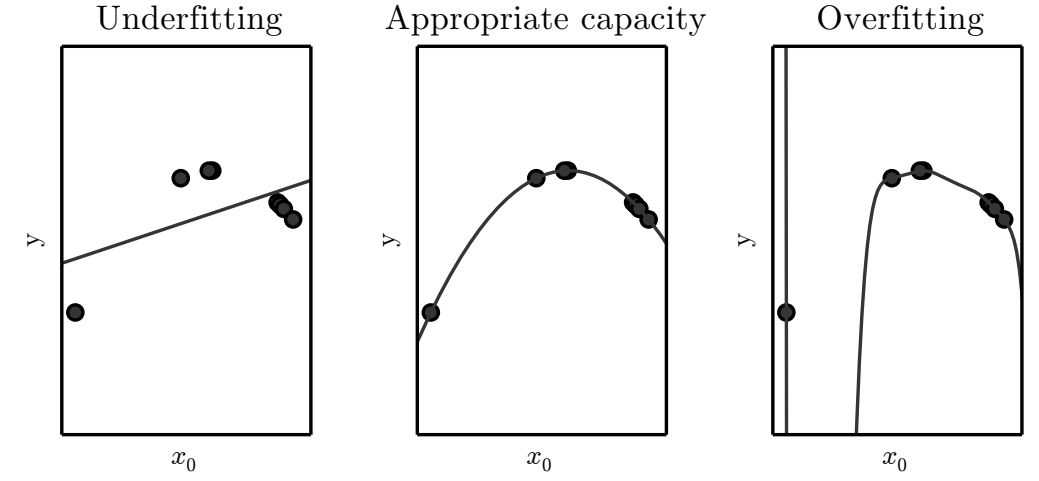
\includegraphics[width=0.6\textwidth]{figure_ml/u_a_o.png}
\end{figure}
\FloatBarrier

Typical method is to check on independent sample for the same process (Or just split your sample in two and use only half for training).

\begin{figure}[ht]
	\centering
	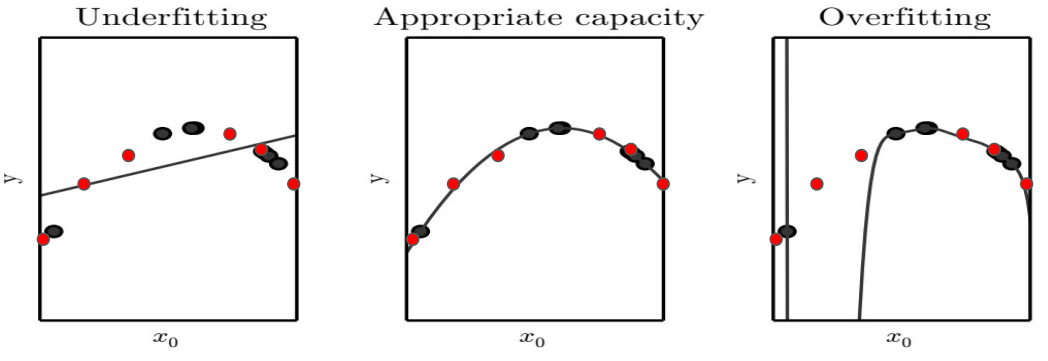
\includegraphics[width=0.6\textwidth]{figure_ml/u_a_o2.png}
\end{figure}
\FloatBarrier

\subsection{Generalization}

We can compare the accuracy between the “training” sample and the “generalization/validation” sample.\\

\begin{figure}[ht]
	\centering
	\begin{subfigure}{.5\textwidth}
		\centering
		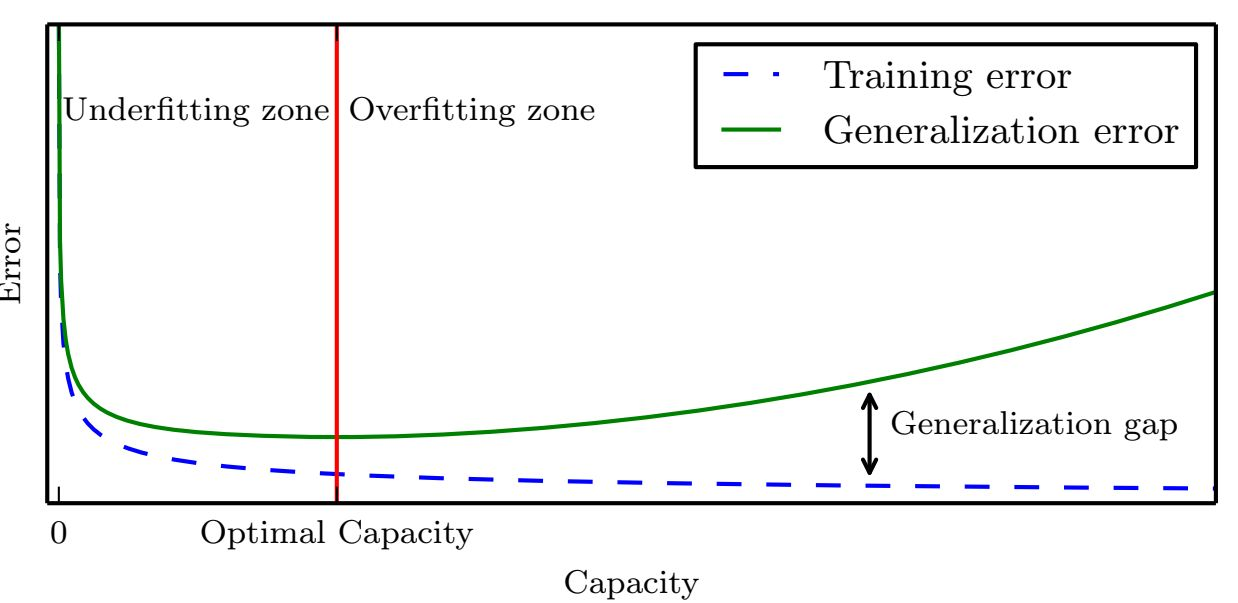
\includegraphics[width=1\linewidth]{figure_ml/generalization.png}
	\end{subfigure}%
	\begin{subfigure}{.5\textwidth}
		\centering
		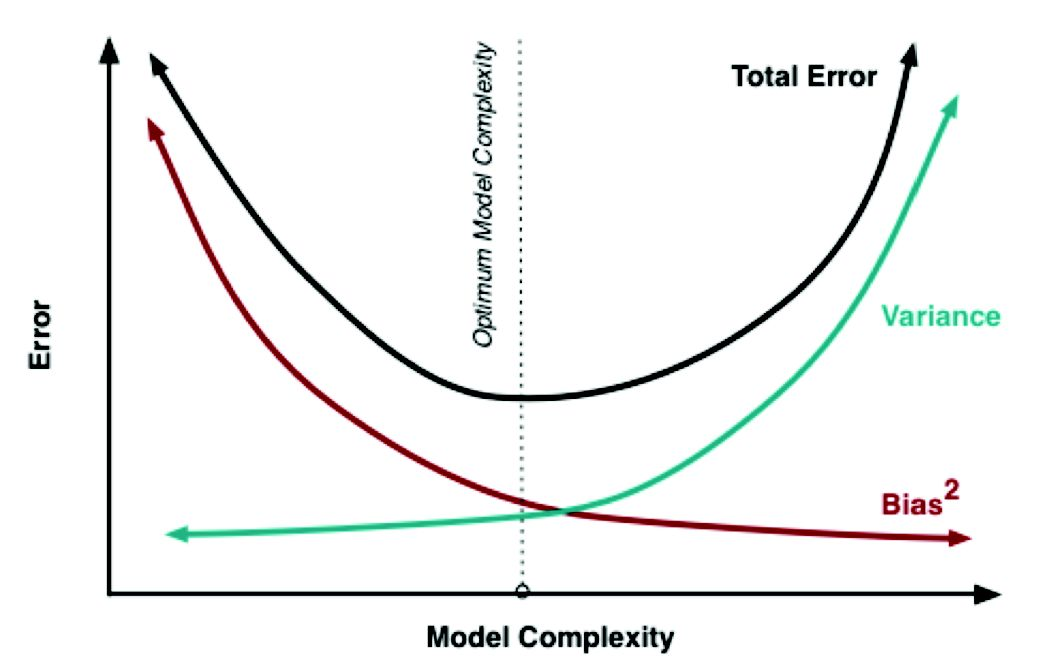
\includegraphics[width=1\linewidth]{figure_ml/generalization2.png}
	\end{subfigure}

\end{figure}



Bias/variance trade-off
\begin{itemize}
	\item y: function (with random noise)
	\item h(x): approximated function
\end{itemize}


\begin{figure}[ht]
	\centering
	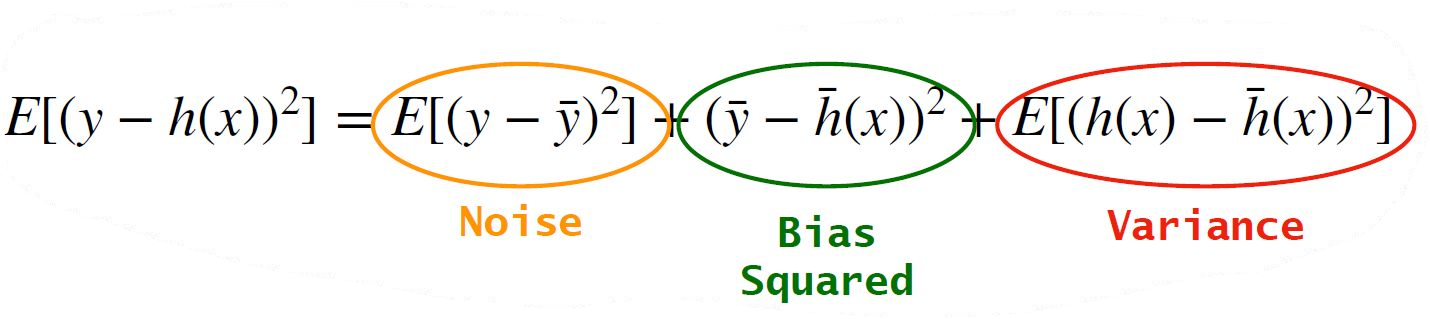
\includegraphics[width=0.45\textwidth]{figure_ml/generalization3.png}
\end{figure}
\FloatBarrier


\subsection{Regularization}

\begin{wrapfigure}{r}{0.45\textwidth}
	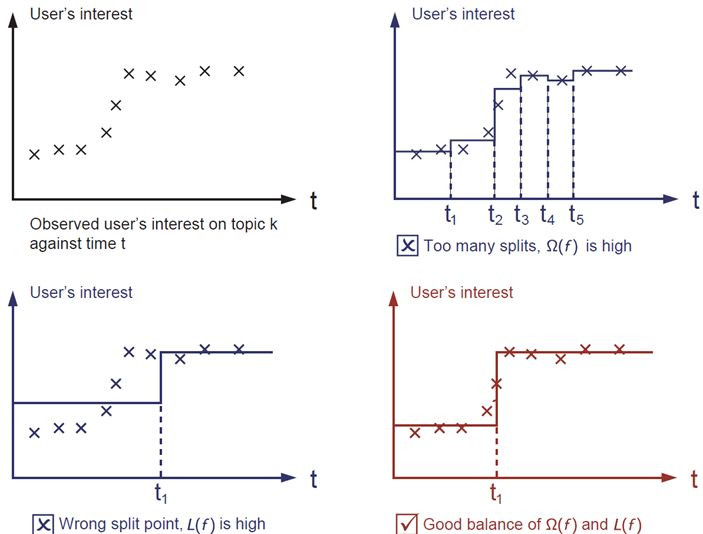
\includegraphics[width=0.45\textwidth]{figure_ml/regularization.png}
\end{wrapfigure} 

Vogliamo evitare che "impari a memoria" il set.\\
In order to control the “generalization gap”. the objective function can be modified adding a regularization term (Introduce a “cost” in increasing the capacity of the model or in accessing some parts of the model-parameters space).\\

the examples in training dataset can be increased with augmentation techniques:

\begin{itemize}
	\item Adding stochastic noise to existing examples
	\item Transforming the existing examples with transformation that are known to be invariant 	for the solution we look for
\end{itemize}


\url{https://xgboost.readthedocs.io/en/latest/tutorials/model.html}



\subsection{Hyperparameters(model) optimization}

It is normal to have to test a few, if not several, configurations in the model hyper-parameter space:
\begin{itemize}
	\item Scans of hyper-parameters are often performed
	\item Different techniques used
\end{itemize}


Effectively a “second” minimization is done

\begin{itemize}
	\item First minimization is on the parameter => minimize on the “training dataset”
	\item Second minimization is on the hyper-parameters => minimize on the “validation dataset”
\end{itemize}

A third dataset (“test dataset”) is then also needed

\begin{itemize}
	\item To assess the performance of the algorithm in an unbiased way
	\item To make an unbiased prediction of the algorithm output
\end{itemize}


Original dataset is typically split in uneven parts to be used as \textit{training}, \textit{validation} and \textit{test}

\begin{figure}[ht]
	\centering
	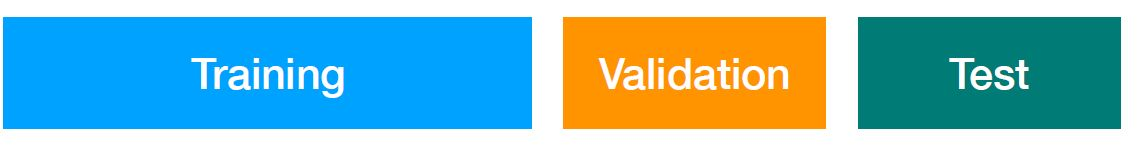
\includegraphics[width=0.7\textwidth]{figure_ml/hyperparams_optimization.png}
\end{figure}
\FloatBarrier

\subsection{K-folding cross validation}

If the sample is statistically limited, splitting in 3 chunks means loosing
examples.\\
With K-folding, “K” independent trainings are performed, each using a
different chunk of data for “training” and for “testing” (and another one for
validation if a hyper parameter scan is performed)

\begin{figure}[ht]
	\centering
	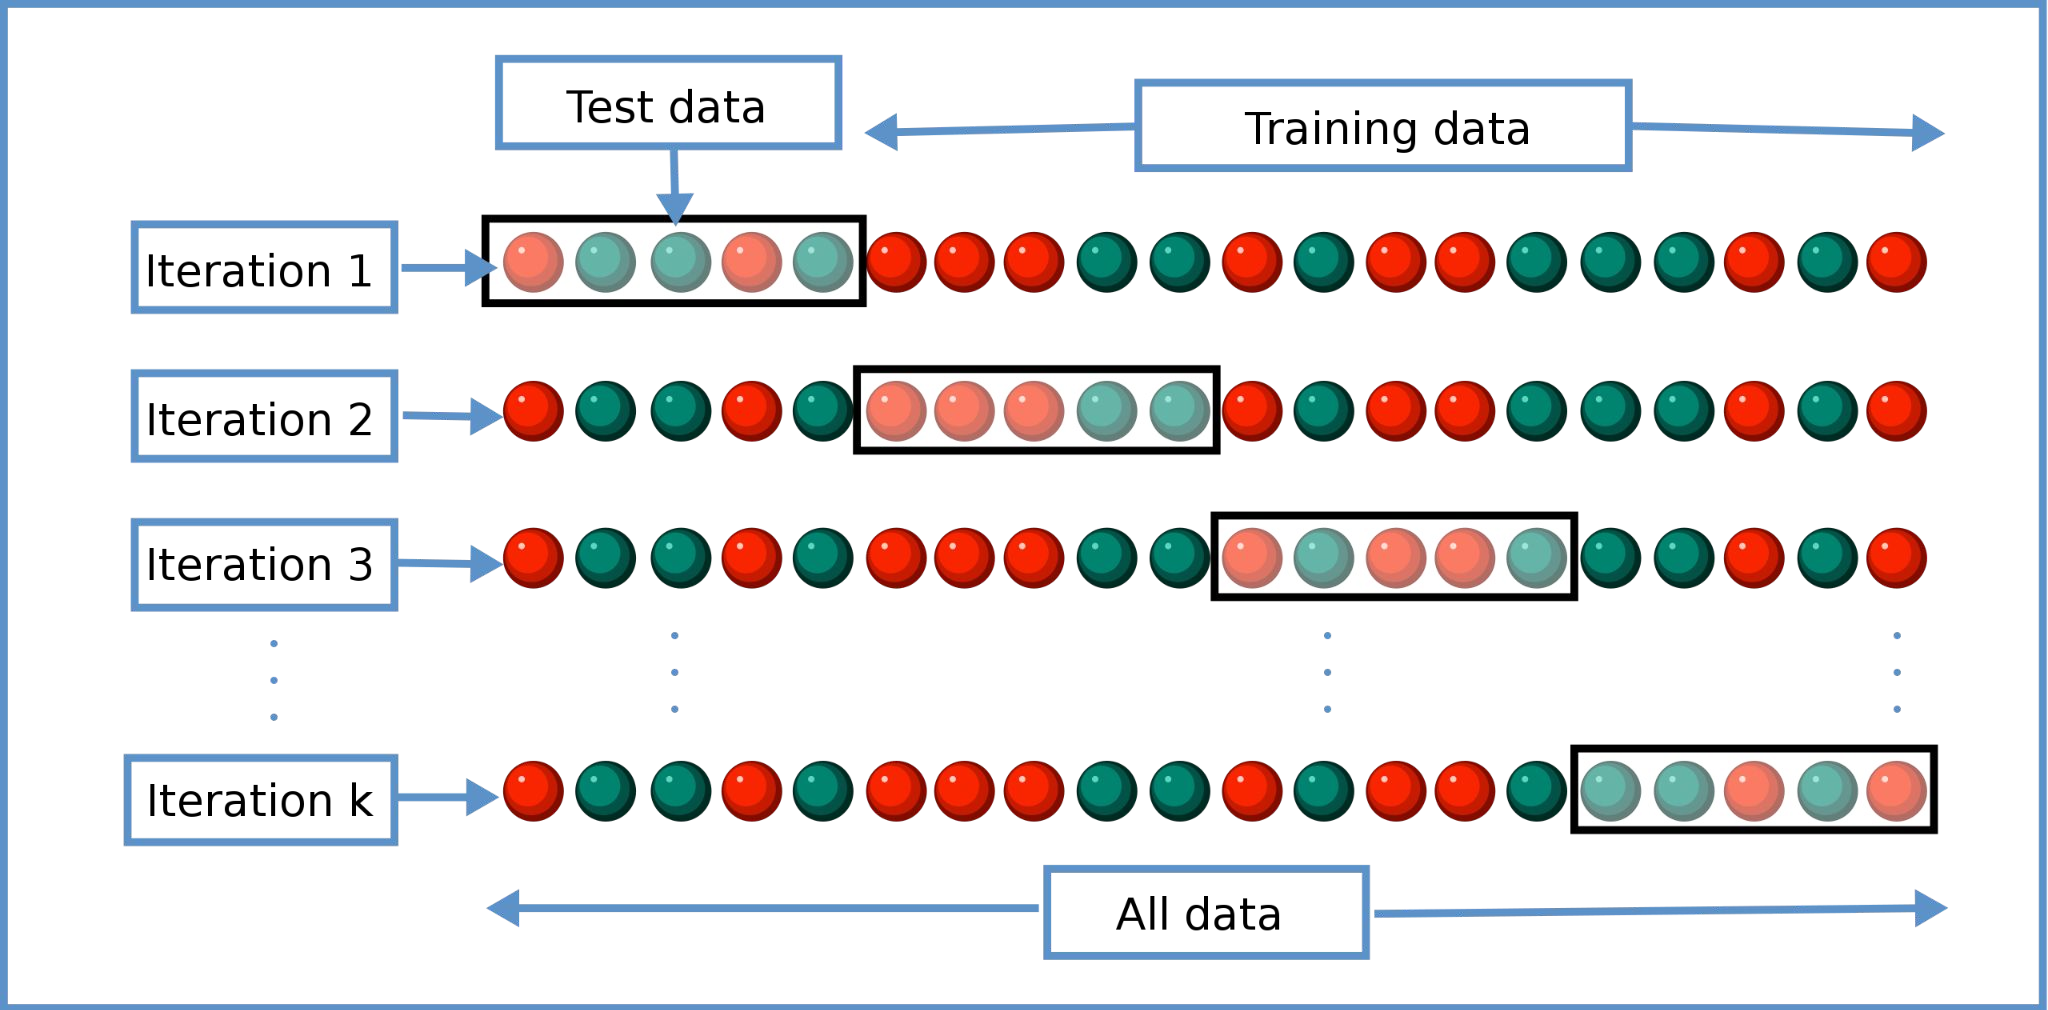
\includegraphics[width=0.7\textwidth]{figure_ml/k-folding.png}
	\caption{Nella figura i dati sono divisi solo in 2 (test e training), ma si possono dividere in 3 come abbiamo visto prima}
\end{figure}
\FloatBarrier

\subsection{Inference}

A ML model that has been trained can than be used to act on some new data (or on the test dataset if a prediction has to be made).
The evaluation of the algorithm output on the “unseen” data is called inference. From a computing time point of view inference is usually much faster than training.

\subsection{Accuracy, Precision, Sensitivity, Specificity}

\begin{figure}[ht]
	\centering
	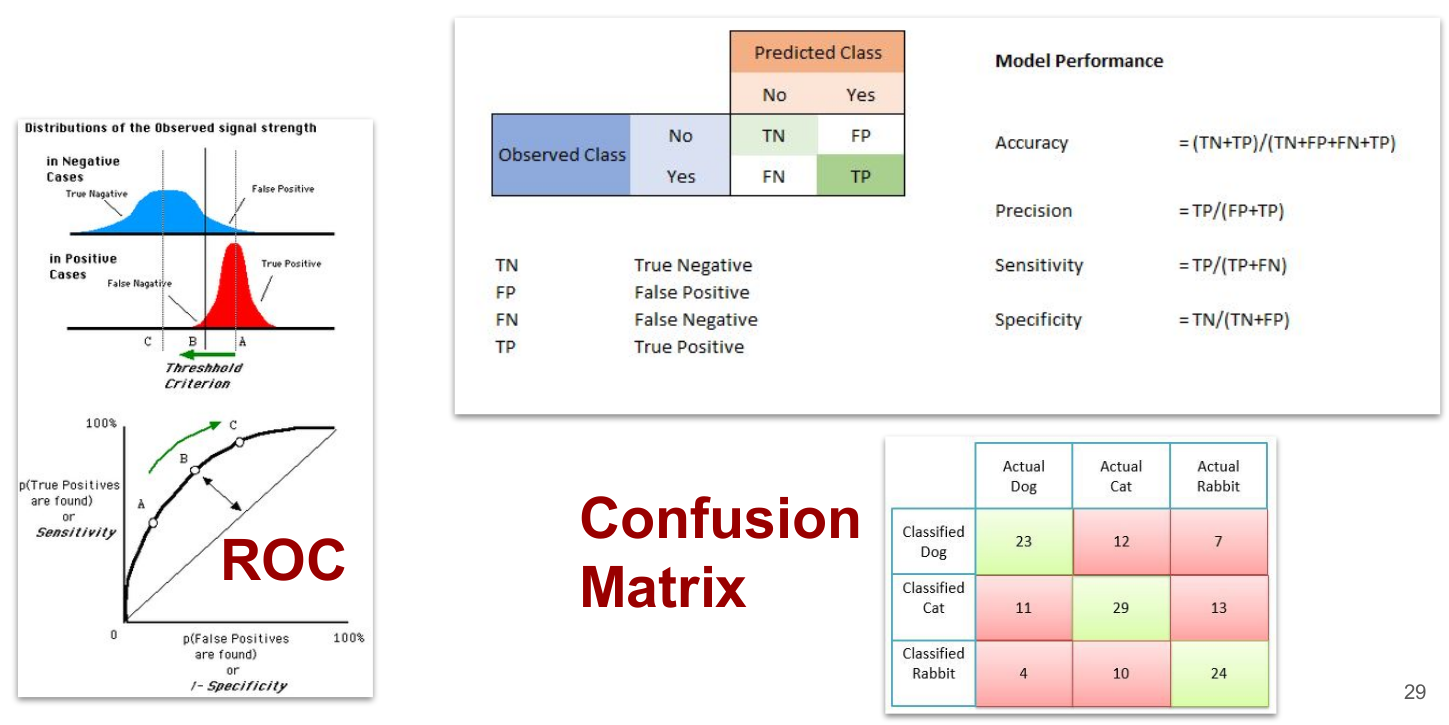
\includegraphics[width=1\textwidth]{figure_ml/apss.png}
\end{figure}
\FloatBarrier


\section{Examples of ML techniques}

\subsection{Linear regression (Supervised)}

Solve a regression problem, i.e. predict the value of y when \textbf{x} is given. Approximate an unknown “y=f(\textbf{x})” given some examples of (y,\textbf{x})\\

\textbf{Model:} $y=w_ix_i$ , i.e. the function is a linear combination of the input parameters\\

\textbf{Parameters:} $ w_i$\\

Let’s suppose we have m examples in the form of pairs $(\textbf{x},y)_j$\\

The \textbf{objective function} can be the mean squared error, MSE=$|y_j - w_i x_{ij} |^2/m$\\

\textbf{Training}: find the parameters $w_i$ that minimize the MSE on the given dataset. Linear regression have an analytical solution (i.e. a minimum for the MSE) that can be computed by requiring the gradient of the MSE to be zero (if you want to see the math \url{https://en.wikipedia.org/wiki/Linear_regression#Least-squares_estimation_and_related_techni
ques}.

We could increase the \textbf{capacity} of the model using polynomials instead of linear functions.The number of parameters would increase as we now would have the second order
coefficients too
\subsection{Principal Component Analysis (aka PCA) (Unsupervised)}

\begin{wrapfigure}{r}{0.45\textwidth}
	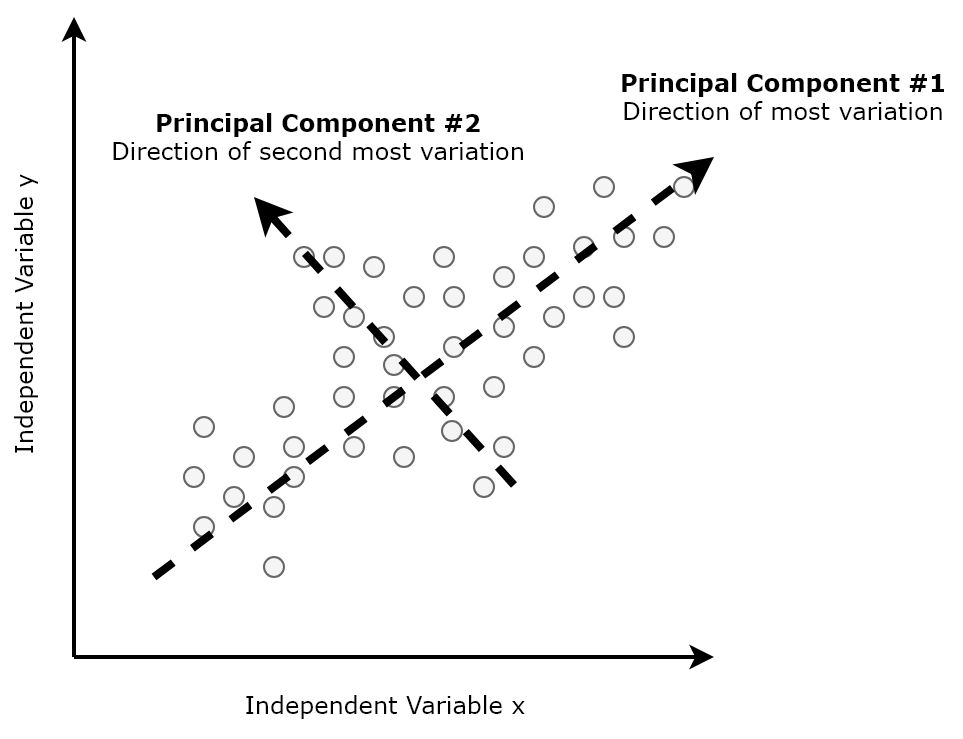
\includegraphics[width=0.45\textwidth]{figure_ml/pca.png}
\end{wrapfigure} 

Orthogonal transformation of the input phase space such that
\begin{itemize}
	\item The first transformed coordinate has maximum variance 
	\item The 2nd transformed coordinated has 2nd max variance
	\item etc.
\end{itemize}

Can be computed as the eigenvalue decomposition of the
covariance matrix

\begin{figure}[ht]
	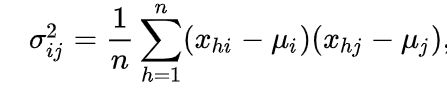
\includegraphics[width=0.35\textwidth]{figure_ml/pca_covariance.png}
\end{figure}
\FloatBarrier

Useful to transform the data in a normalized form (scaling by the variance of each component).\\
Reduce dimensionality (by taking only first N components) capturing only the largest deviations from the mean value.\\

More complex dimensionality reduction Manifold Learning:\url{https://github.com/jakevdp/PythonDataScienceHandbook/blob/master/notebooks/05.10-Manifold-Learning.ipynb}

\subsubsection{Nearest neighbors}

A very powerful way to do classification or regression is to look at points in the training datasets that are close to sample
to evaluate.
Multiple neighbors can be used for
a more stable evaluation.
On large dataset it could be a problem to keep all training points for the evaluation phase.


\begin{figure}[ht]
	\centering
	\begin{subfigure}{.5\textwidth}
		\centering
		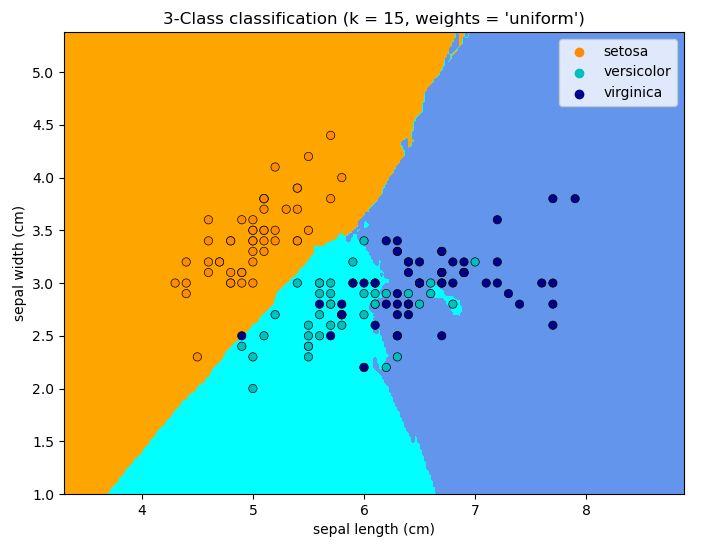
\includegraphics[width=1\linewidth]{figure_ml/nn.png}
	\end{subfigure}%
	\begin{subfigure}{.5\textwidth}
		\centering
		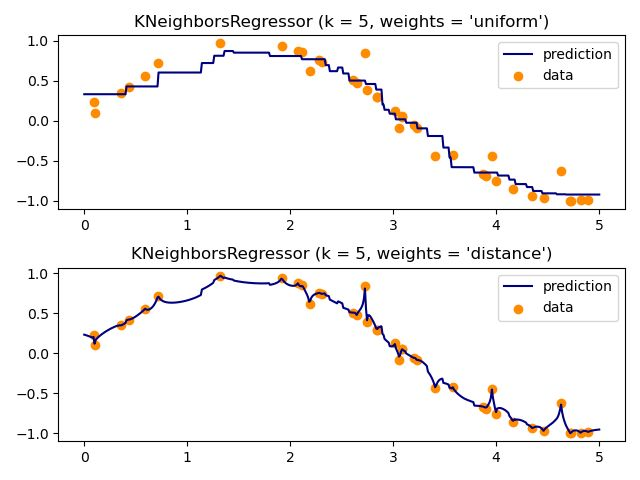
\includegraphics[width=1\linewidth]{figure_ml/nn2.png}
	\end{subfigure}
	\caption{
		Figures from \url{https://scikit-learn.org/stable/modules/neighbors.html}.
	}
\end{figure}


\subsection{Decision trees}

The functions used in the “model” are decision trees, each node has a pass/fail condition on some input variable.\\
Classification and regression trees (CART)
\begin{itemize}
	\item Examples are categorized based on individual “cuts” on a single input feature
	\item A score is given in each leaf
\end{itemize}
Trees can have different depths (depth is an hyper-parameter)

\begin{figure}[ht]
	\centering
	\begin{subfigure}{.5\textwidth}
		\centering
		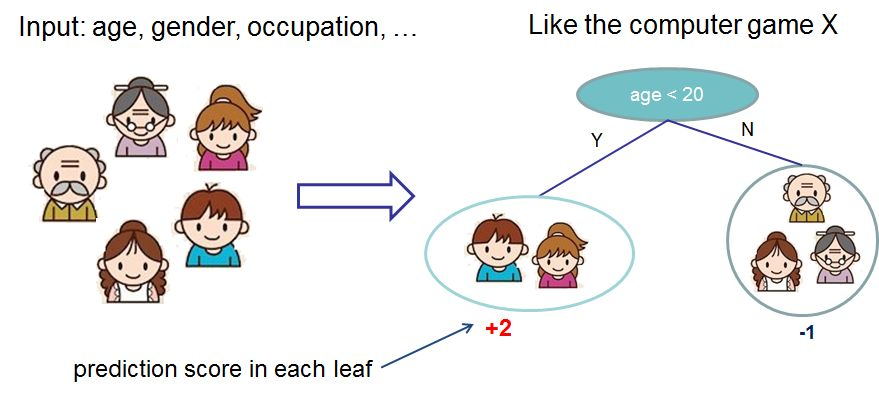
\includegraphics[width=1\linewidth]{figure_ml/decision_trees.png}
	\end{subfigure}%
	\begin{subfigure}{.5\textwidth}
		\centering
		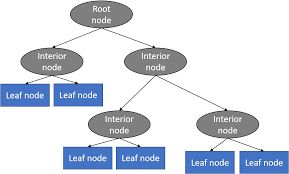
\includegraphics[width=1\linewidth]{figure_ml/decision_trees2.png}
	\end{subfigure}
\end{figure}



\url{https://xgboost.readthedocs.io/en/latest/tutorials/model.html}


\subsection{Ensembles of trees}

A single tree is typically not a very performant.\\
Combine multiple trees (\#trees is an hyperpar)
\begin{itemize}
	\item Random forest (bagging)
	\item Gradient boosting
	\item Adaptive boosting
\end{itemize}

\begin{figure}[ht]
	\centering
	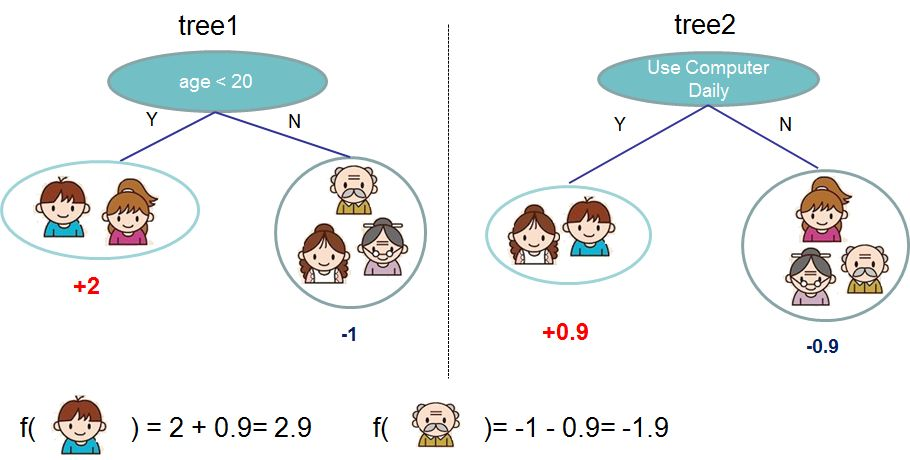
\includegraphics[width=0.5\textwidth]{figure_ml/trees.png}
\end{figure}
\FloatBarrier

\begin{figure}[ht]
	\centering
	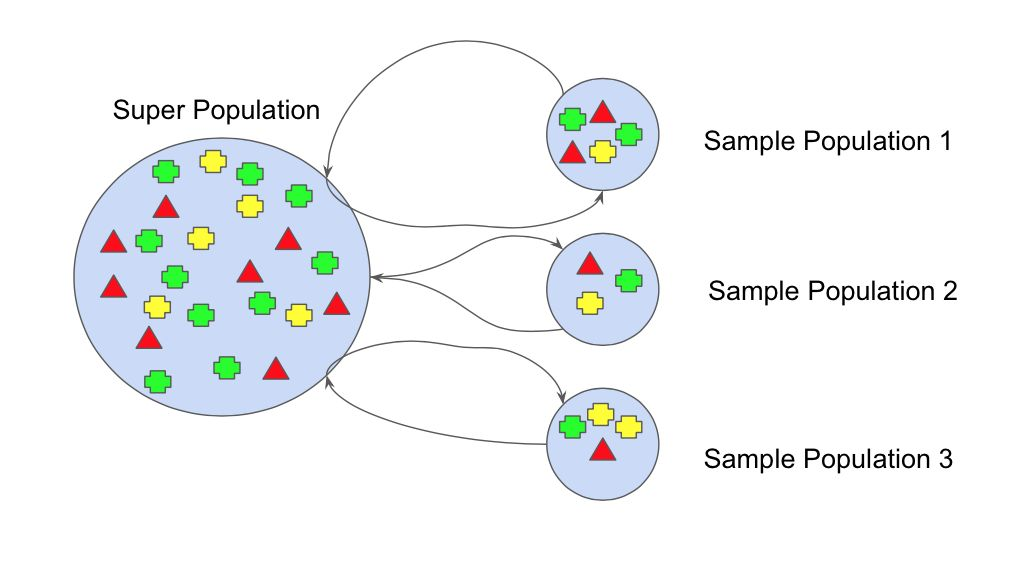
\includegraphics[width=0.5\textwidth]{figure_ml/bagging.png}
\end{figure}
\FloatBarrier

\begin{figure}[ht]
	\centering
	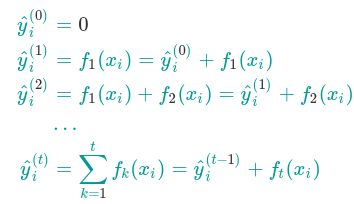
\includegraphics[width=0.5\textwidth]{figure_ml/g_b.png}
\end{figure}
\FloatBarrier

\begin{figure}[ht]
	\centering
	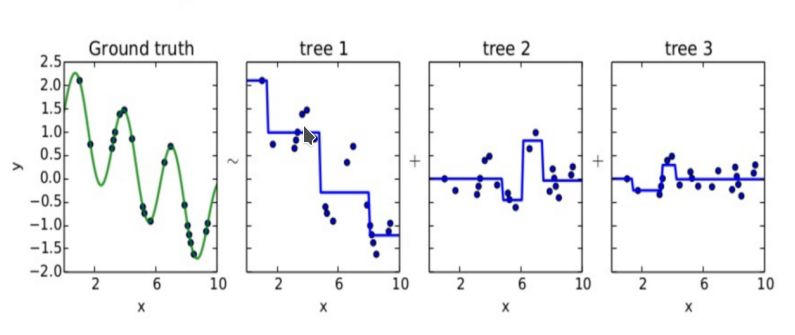
\includegraphics[width=0.5\textwidth]{figure_ml/g_b2.png}
\end{figure}
\FloatBarrier

\subsection{Limitations of decision trees}
Cuts are axis aligned!\\
Classification of \textbf{x1 > x2} is a hard problem for a decision tree

\begin{figure}[ht]
	\centering
	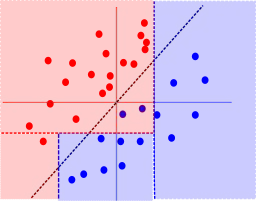
\includegraphics[width=0.4\textwidth]{figure_ml/limitations_trees.png}
\end{figure}
\FloatBarrier

\begin{figure}[ht]
	\centering
	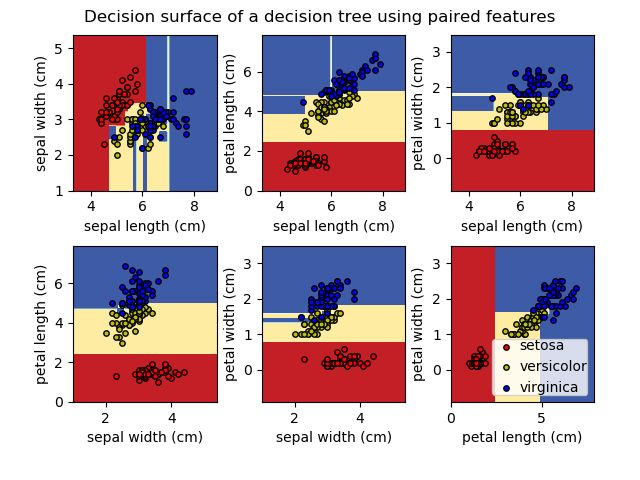
\includegraphics[width=0.5\textwidth]{figure_ml/limitations_trees2.png}
\end{figure}
\FloatBarrier

\subsection{Many more ML techniques!}

Scikit-learn library offers many ML techniques implementation in python.\\
\url{https://scikit-learn.org/stable/auto_examples/classification/plot_classifier_comparison.html#sphx-glr-auto-examples-classification-plot-classifier-comparison-py}

\begin{figure}[ht]
	\centering
	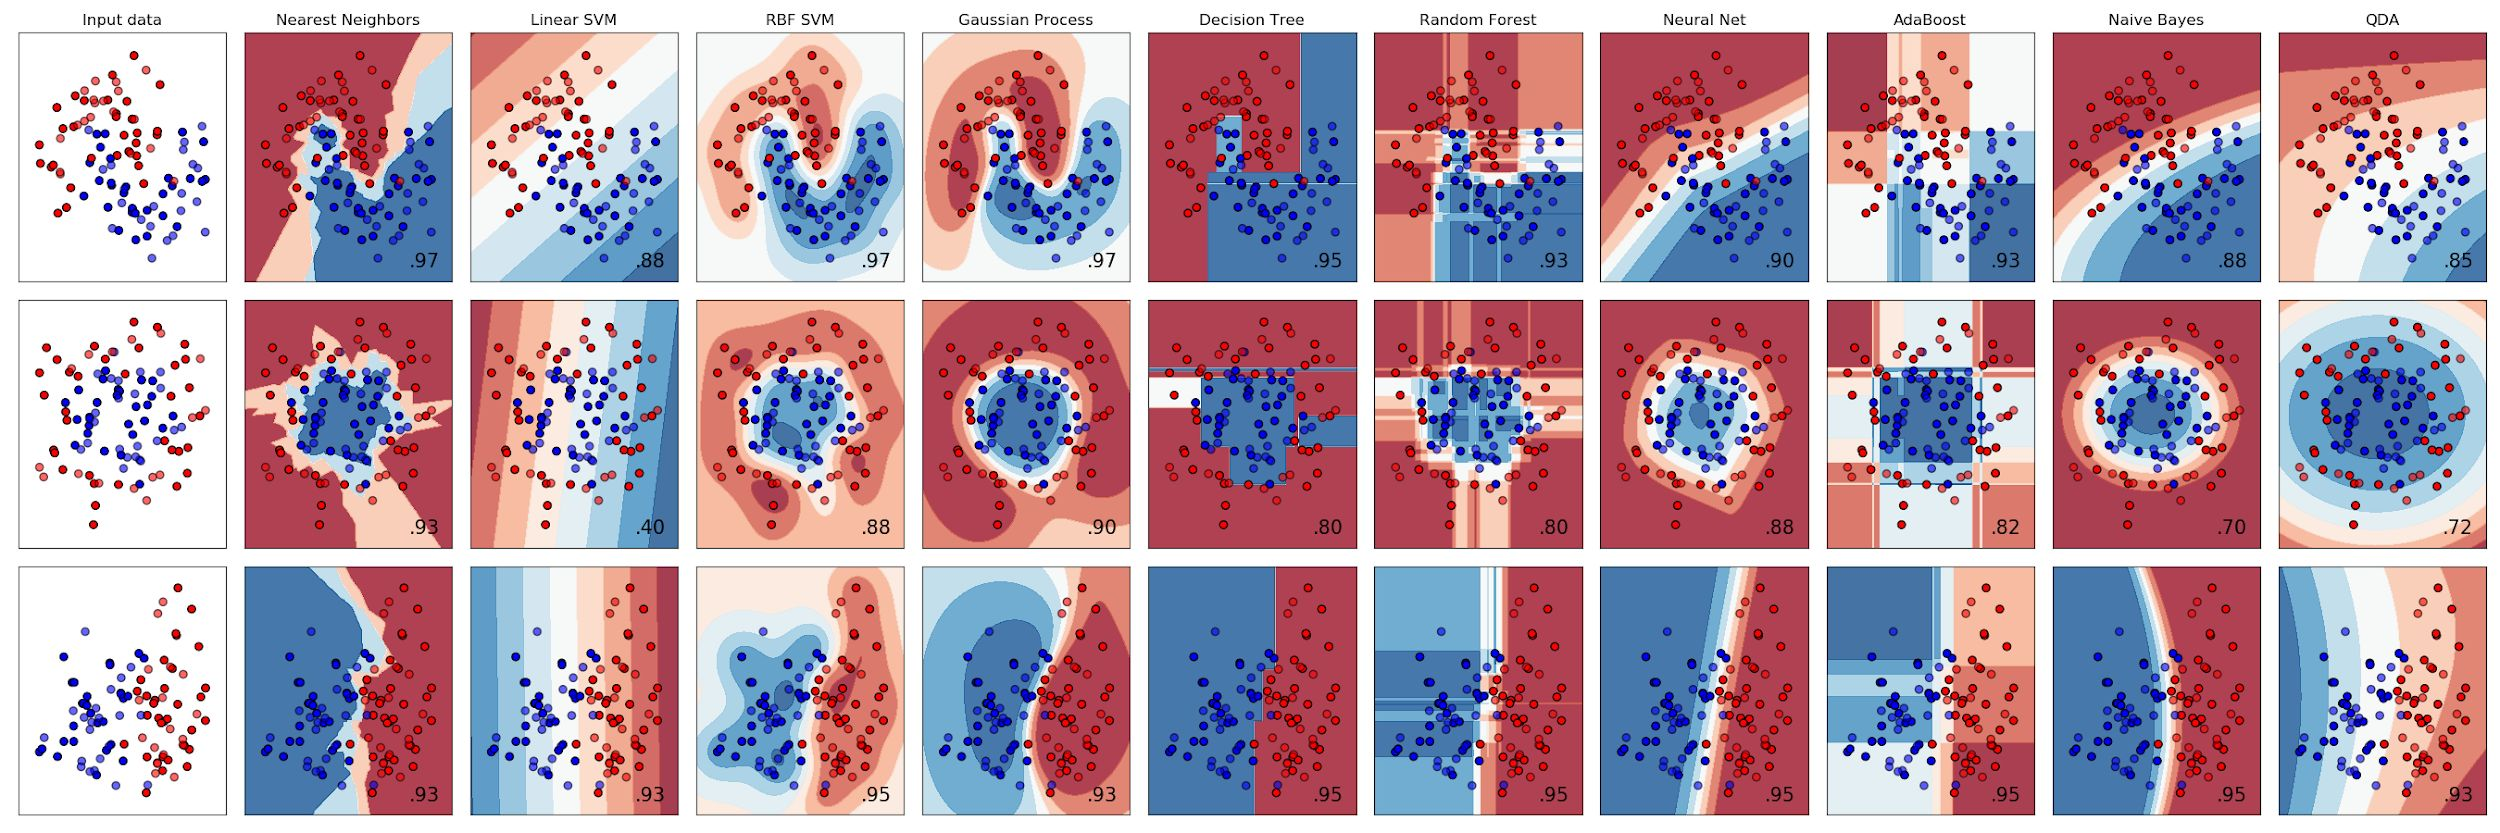
\includegraphics[width=0.5\textwidth]{figure_ml/scikit.png}
\end{figure}
\FloatBarrier

\subsection{What do we need to create our first ML program}

-Load some data
\begin{itemize}
	\item We use numpy arrays as data structures, today we load data from some existing repositories
	\item We need an “X” and a “y” array for input data and for labels (for a supervised algorithm)
	\item Different examples on the same dataset are placed in ROWS
	\begin{itemize}
		\item Rows are corresponding to the first index in numpy multi index array (aka tensor)
		\item Columns correspond to different “input features”
	\end{itemize}
\end{itemize}

-Use some existing library implementing a ML algorith (Python library exists for almost any ML algorithm).\\

-Feed the data to the library (We need to understand for each library how you run the “training” step)\\

Check the result: We need to understand how to do the inference of a trained model, for example on a new sample or on a new dataset.


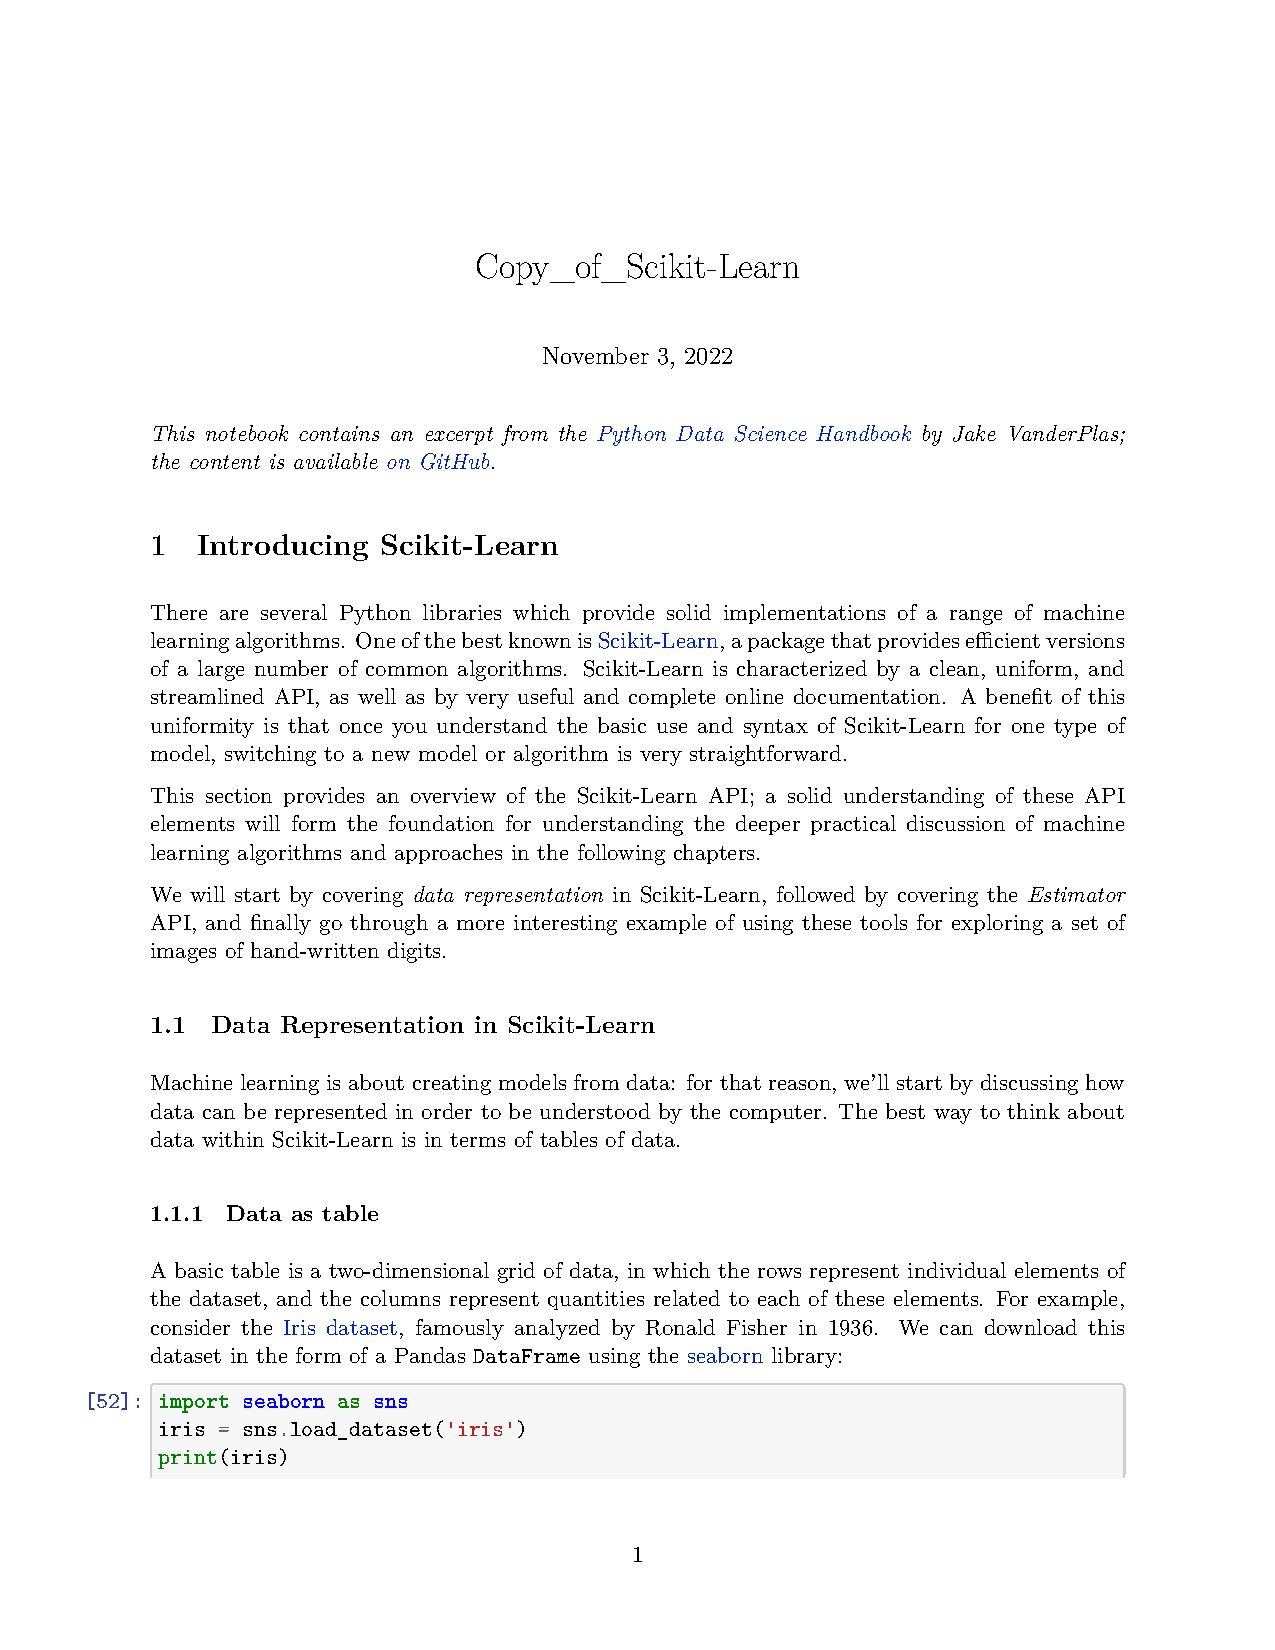
\includepdf[pages=-]{Copy_of_Scikit-Learn.pdf}
